\documentclass{tufte-handout}

\usepackage{graphicx,amsmath,amsfonts}

\title{Probability Distributions}
\author{}
\date{}

\begin{document}
\maketitle

\section{Binomial Distribution}
\begin{figure}
    \caption{Binomial Distribution}
    \centering
    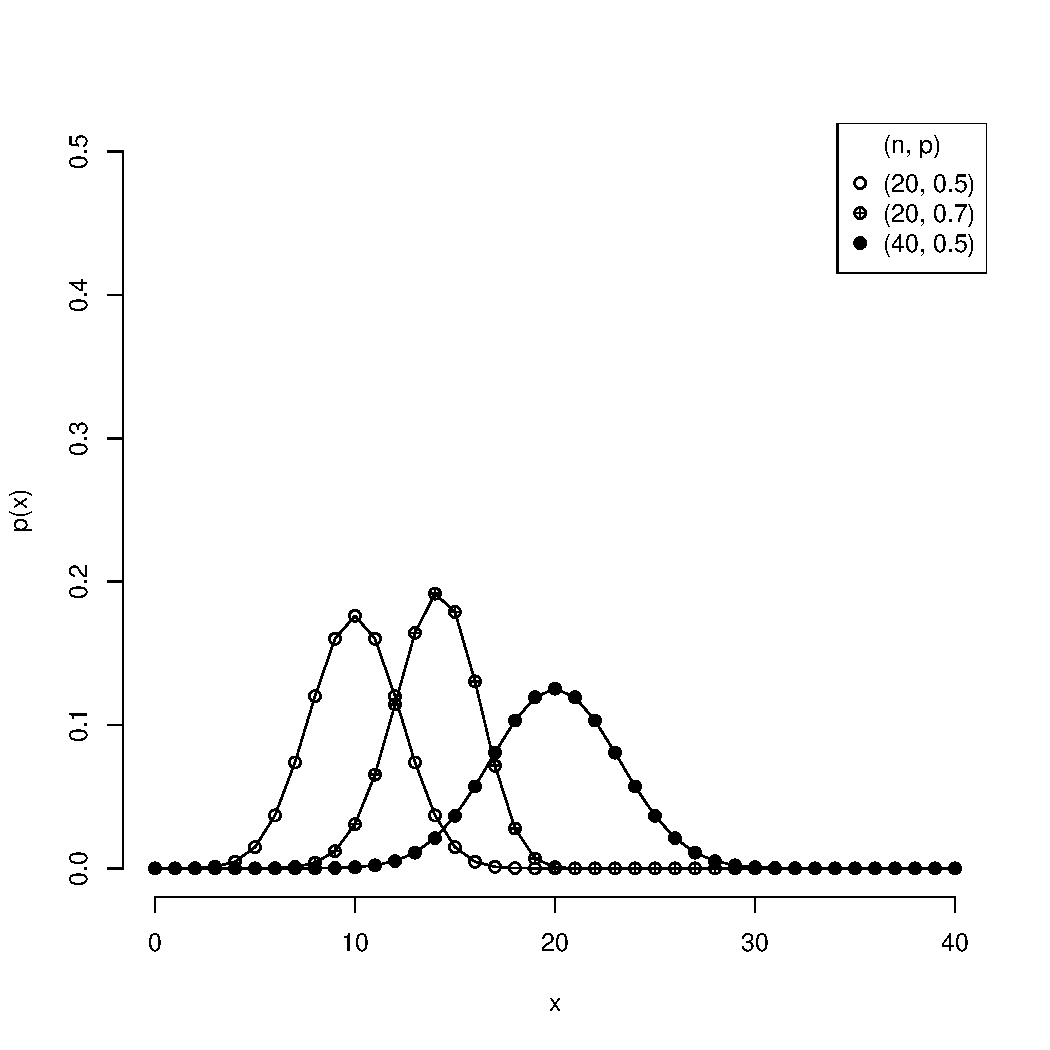
\includegraphics[width=.70\textwidth]{../distributions/binomial/binomial_bw.pdf}
\end{figure}
\marginnote[-3.0in]{
    \begin{align*}
        & X \sim \text{Binomial} (n, p) \\
        & p \in (0, 1) \\
        & x = 0, 1, 2, \dots, n \\
        \\
        & f(x) = {n \choose x} p^x (1-p)^{x-1} \\
        & \mu = E[X] = np \\
        & \sigma^2 = E[(x-\mu)^2] = np(1-p) \\
        \\
        & M(t) = [pe^t + (1-p)]^n & t\in\mathbb{R} \\
    \end{align*}
}

\section{Poisson Distribution}
\begin{figure}
    \caption{Poisson Distribution}
    \centering
    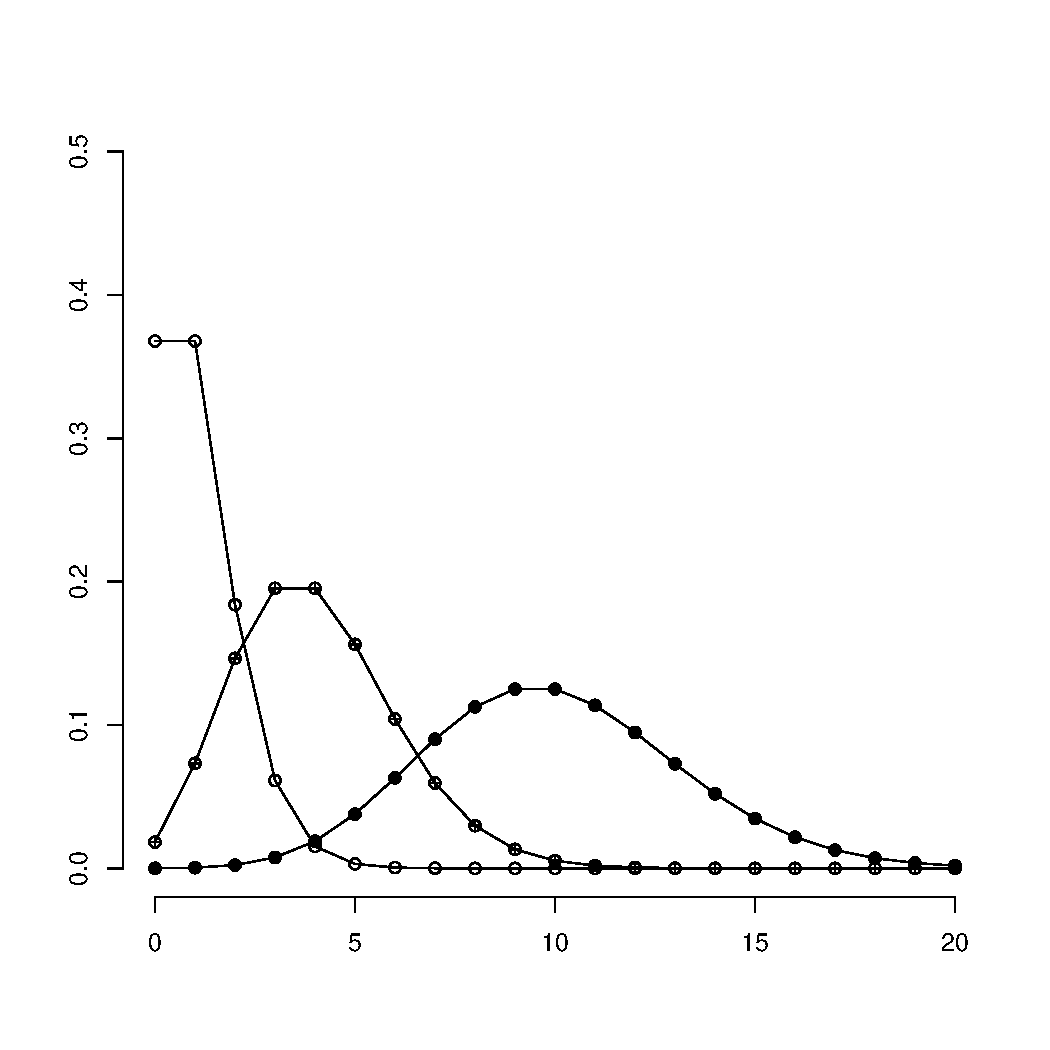
\includegraphics[width=.70\textwidth]{../distributions/poisson/poisson_bw.pdf}
\end{figure}
\marginnote[-3.0in]{
    \begin{align*}
        & X \sim \text{Poisson} (\lambda) \\
        & \lambda \in \mathbb{R^+} \\
        & x = 0, 1, 2, \dots \\
        \\
        & f(x) = \frac{e^{-\lambda}\lambda^x}{x!} \\
        & \mu = E[X] = \lambda \\
        & \sigma^2 = E[(x-\mu)^2] = \lambda \\
        \\
        & M(t) = e^{\lambda (t-1)} & t \in \mathbb{R} \\
    \end{align*}
}

\newpage

\section{Normal Distribution}
\begin{figure}
    \caption{Normal$(0,1)$ Distribution}
    \centering
    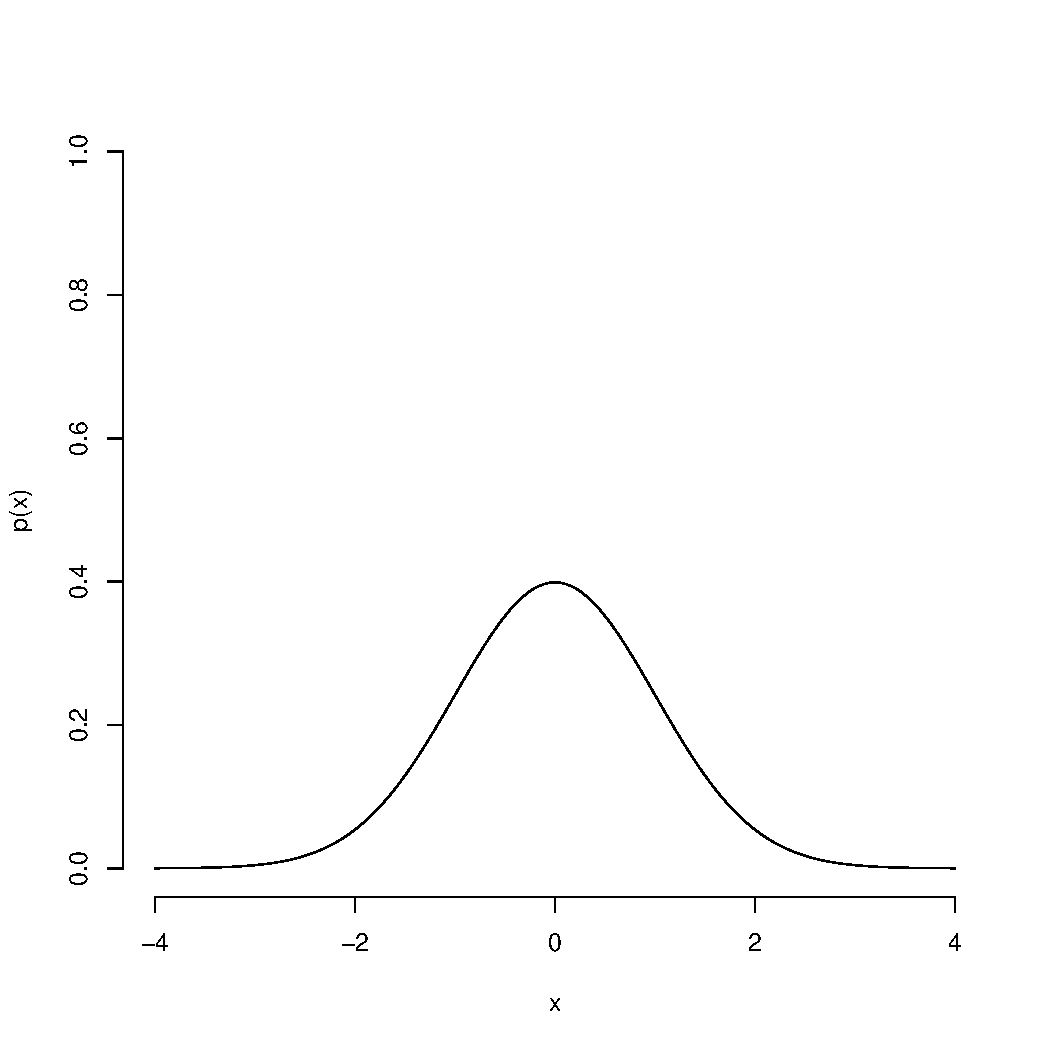
\includegraphics[width=.70\textwidth]{../distributions/normal/normal_bw.pdf}
\end{figure}
\marginnote[-3.0in]{
    \begin{align*}
        & X \sim \text{Normal} (\mu, \sigma^2) \\
        & \mu \in \mathbb{R} \\
        & \sigma^2 \in \mathbb{R^+}\\
        & x \in \mathbb{R} \\
        \\
        & f(x) = \frac{1}{\sqrt{2\pi\sigma^2}}\exp\left[-\frac{(x
            -\mu)^2}{2\sigma^2} \right] \\
        & \mu = E[X] = \mu \\
        & \sigma^2 = E[(x-\mu)^2] = \sigma^2 \\
        \\
        & M(t) = e^{\mu t + \frac{1}{2} \sigma^2 t^2} & t \in \mathbb{R} \\
    \end{align*}
}

\end{document}
